\subsection{Harmoniske svingninger}\label{teori: Harmoniske svingninger}
En oscillerende bevægelse er en bevægelse hvor et objekt vil bevæge sig frem og tilbage over sin hviletilstand. Dette kan eksempelvis ses hos penduler og masser bundet til fjedre.
\\

\begin{wrapfigure}{r}{0.3\textwidth}
\centering
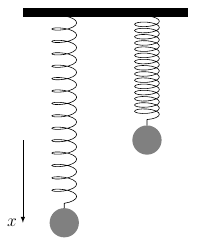
\includegraphics[scale=1]{Billeder/fjeder}
\caption{Fjeder med lod \label{fig:fjeder}}
\end{wrapfigure} 

Eksemplet der vil blive betragtet i dette kapitel, er en oscillerende bevægelse, som er hensigtsmæssig se på i forhold til at forstå principperne bag IR-spektroskopi. Der  vil blive set på et objekt med en masse, som er bundet til en fjeder. se figur \ref{fig:fjeder}.

Med udgangspunkt i figur \ref{fig:fjeder} vil vi se på en fjeder, der i den ene ende er fastgjort til noget stationært og i den anden ende er fastgjort til en kugle. Når kuglen ikke påvirkes af andre ydre kræfter end tyngdekraften, vil kuglen opnå en hviletilstand hvor fjederkraften er lige så stor som tyngdekraften. Vi sætter denne hviletilstand til $x_0=0$. Når systemet påvirkes af en ydre kraft, f.eks. at kuglen bliver hivet i, vil fjederen svare tilbage med at trække endnu hårdere i kuglen. Hvis vi betrager opad som den positive retning vil vi på figur \ref{fig:fjeder} have flyttet kuglen en afstand $-x$ væk fra sin hvileposition og fjederkraften givet ved Hookes lov, der blev beskrevet i \ref{Hookes} vil være lig $F_x=-k \cdot -x$. Hvor F er fjederkraften, k er fjederkonstanten for den givne fjeder og x er afstanden flyttet fra hvilepositionen $x_0$. Hvis der var interesse for, at vide hvor kuglen befandt sig til et tidspunkt, t, ville vi være nød til at have en positionsfunktion, som kunne give os den viden. Denne funktion vil nu blive udledt.